\documentclass[Main.tex]{AspectRatio.tex}
\begin{document}
\chapter{Aspekt ratio}

Aspekt ratio refererer til den proportionelle forskel mellem en skærms højde og brede \cite{Gibson}. Der findes mange forskellige aspekt ratios, som bliver brugt til forskellige formål \cite{CommonResolutions}. I dag er de langt mest benyttede opløsning blandt spillere på Steam 1920x1080, efterfulgt af 1366x768. Begge disse opløsninger er 16:9 formater. Andre formater der udgør en betydelig del er 1280x1024 (5:4), 1680x1050 (16:10), og 1440x900 (16:10) \cite{Steam}.

At skifte mellem to forskellige opløsninger, som deler det samme aspekt ratio, er relativt simpelt, da teksturer blot kan skaleres til at have en anden størrelse. Så længe at ratioen er den samme, og teksturen bliver skaleret ned til en dårligere opløsning, er der generelt ikke et problem. 

Problematikken opstår når at aspekt ratioen ændres, da en skalering ikke længere blot vil ændre på størrelsen af teksturen, men også på forholdet mellem bredden og højde. Det betyder at akserne ikke bliver skaleret synkront, hvilket kan give billedet et andet visuelt indtryk. Dette har været tilfældet i mange ældre spil, der originalt ikke var lavet til widescreen, blandt andet Warcraft 3, som kan ses på figur \ref{Warcraft_4,3} og \ref{Warcraft_16,9}. \cite{Wills}

\begin{figure}[h]
\centering
\parbox{7cm}{   
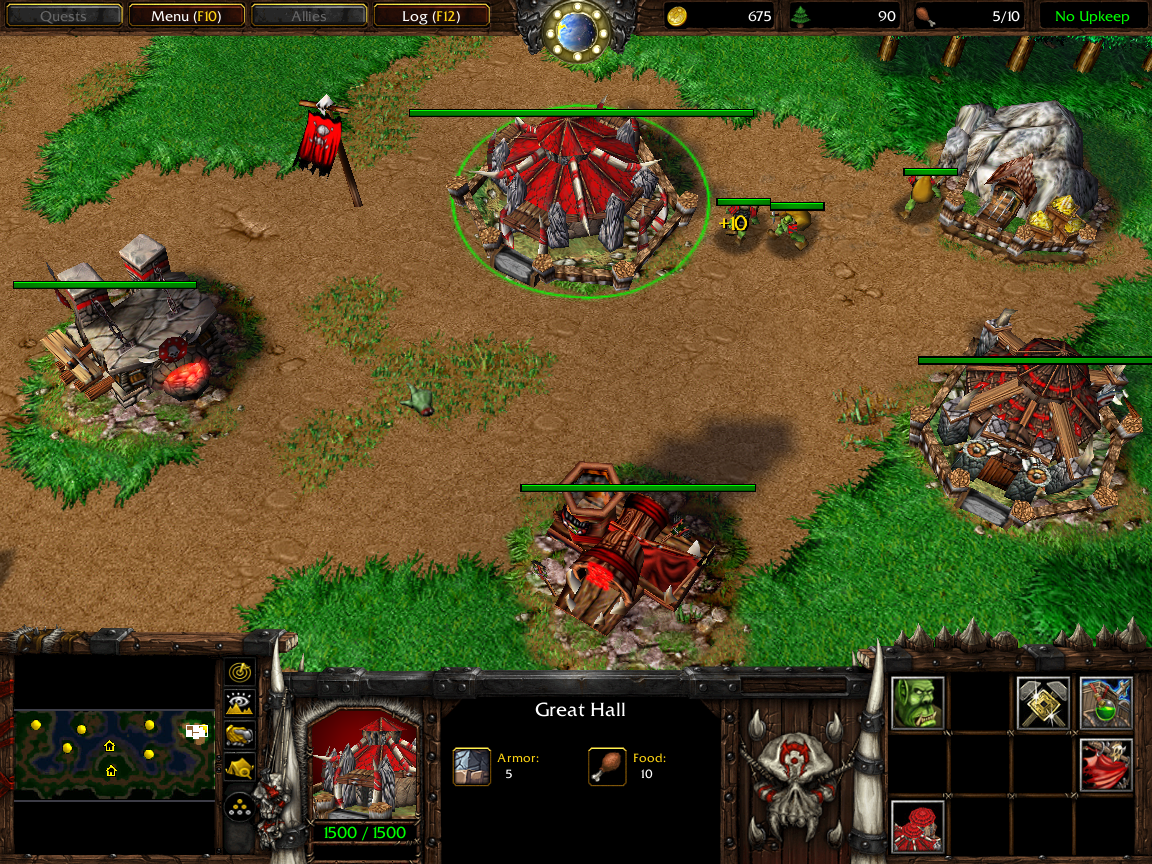
\includegraphics[width = 7cm]{billeder/Warcraft_4,3}
\caption{Warcraft 3 i dets originale 4:3 aspekt ratio}    
\label{Warcraft_4,3}}
\qquad
\begin{minipage}{9.33cm}
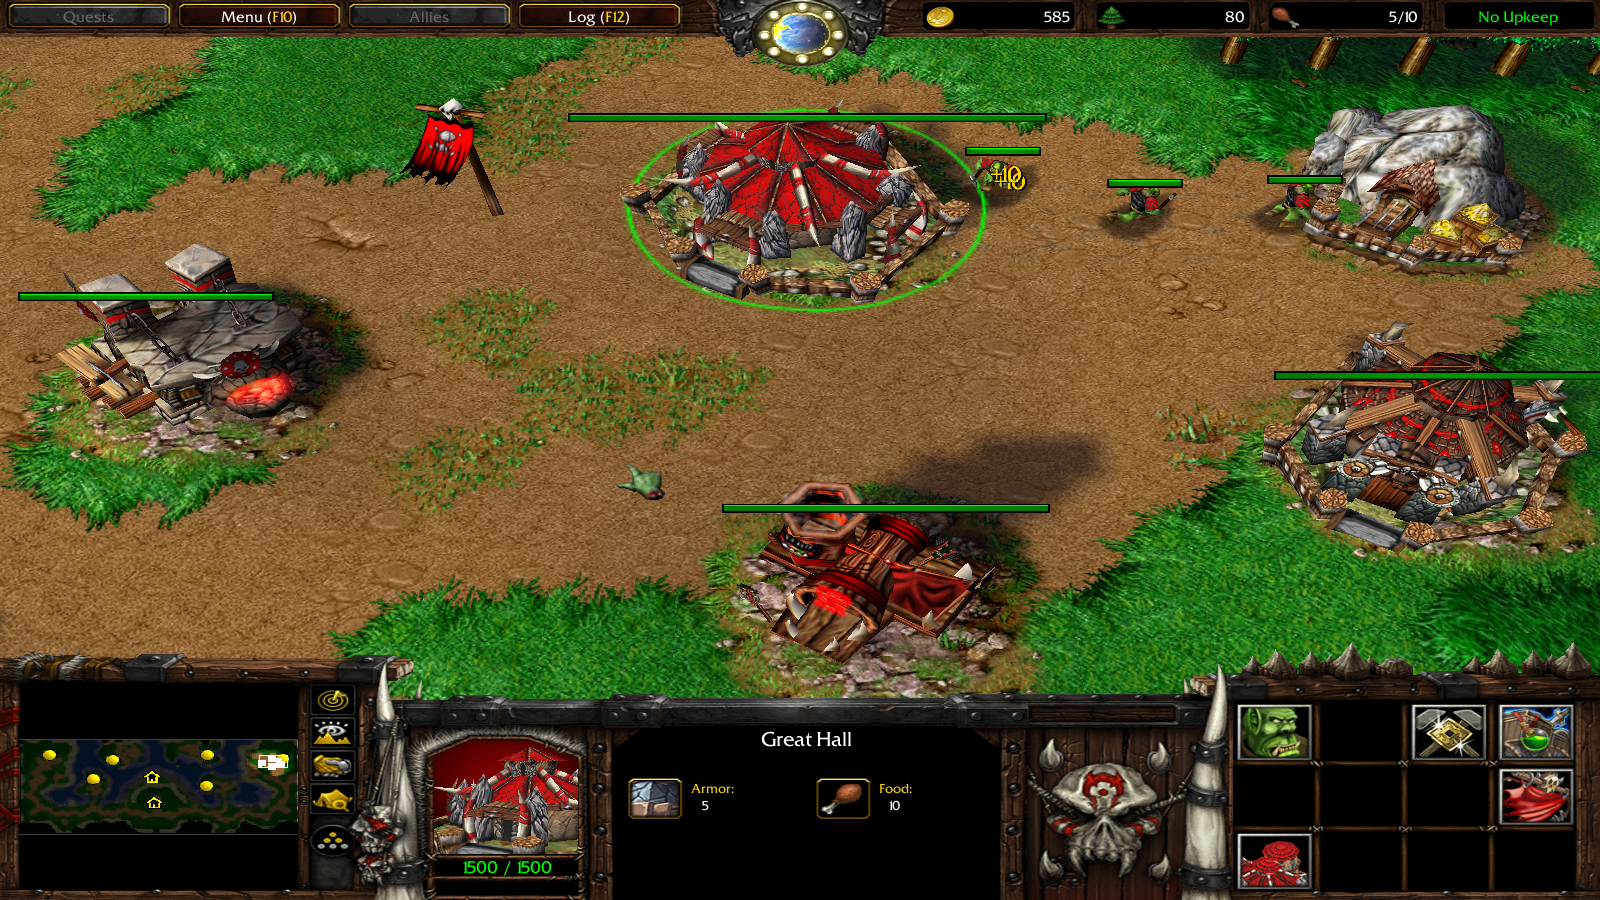
\includegraphics[width = 9.33cm]{billeder/Warcraft_16,9}
\caption{Warcraft 3 skaleret asynkront til et 16:9 aspekt ratio}    
\label{Warcraft_16,9}
\end{minipage}
\end{figure}

\section{Field of View}

Der er to måder at komme uden om dette problem på. Den ene er at ændre på field of view (FOV), som er hvor stor en del at spilleren ser af spilverdenen. Dette bringer imidlertidigt sine egne problemer på banen. Når FOV ændres, ændres der også på det output spilleren får på sin skærm, hvilket betyder at alle spillere ikke ser spilverdenen ens. Hvis at spillet ikke er kompetitivt spil, behøver dette ikke at være en bekymring, da spilleren kun spiller mod sig selv, og spillet i den forstand er ligestillet for alle. Hvis spillet derimod er kompetitivt, medfører det med stor sandsynlighed at spillere med et vist aspekt ratio har en fordel over dem med et andet aspekt ratio \cite{Atwood}.

Hvis vi ser på et 2d spil, og forestiller os et endless runner spil, så som Robot Unicorn Attack, hvor at man kun ser hvad der er lige foran sin karakter, vil et bredere FOV betyde at man har længere til at forberede sig på de forhindringer der kommer forude.

Hvis vi ser på et 3d spil, så som CS:GO, vil et bredere field of view betyde at spilleren kan se længere til siderne. Det vil sige at spillere med et smallere FOV effektivt set har en blind vinkel, som at deres modspillere med et bredere FOV ikke har, hvilket giver en stor fordel når det kommer til at få visuel kontakt med sine fjender. På figur \ref{CS_GO_16,9} ses f.eks. en dør til højre, som ikke kan ses på figur \ref{CS_GO_4,3} pga. forskellen i FOV.
\clearpage


\begin{figure}[h]
\centering
\parbox{7cm}{
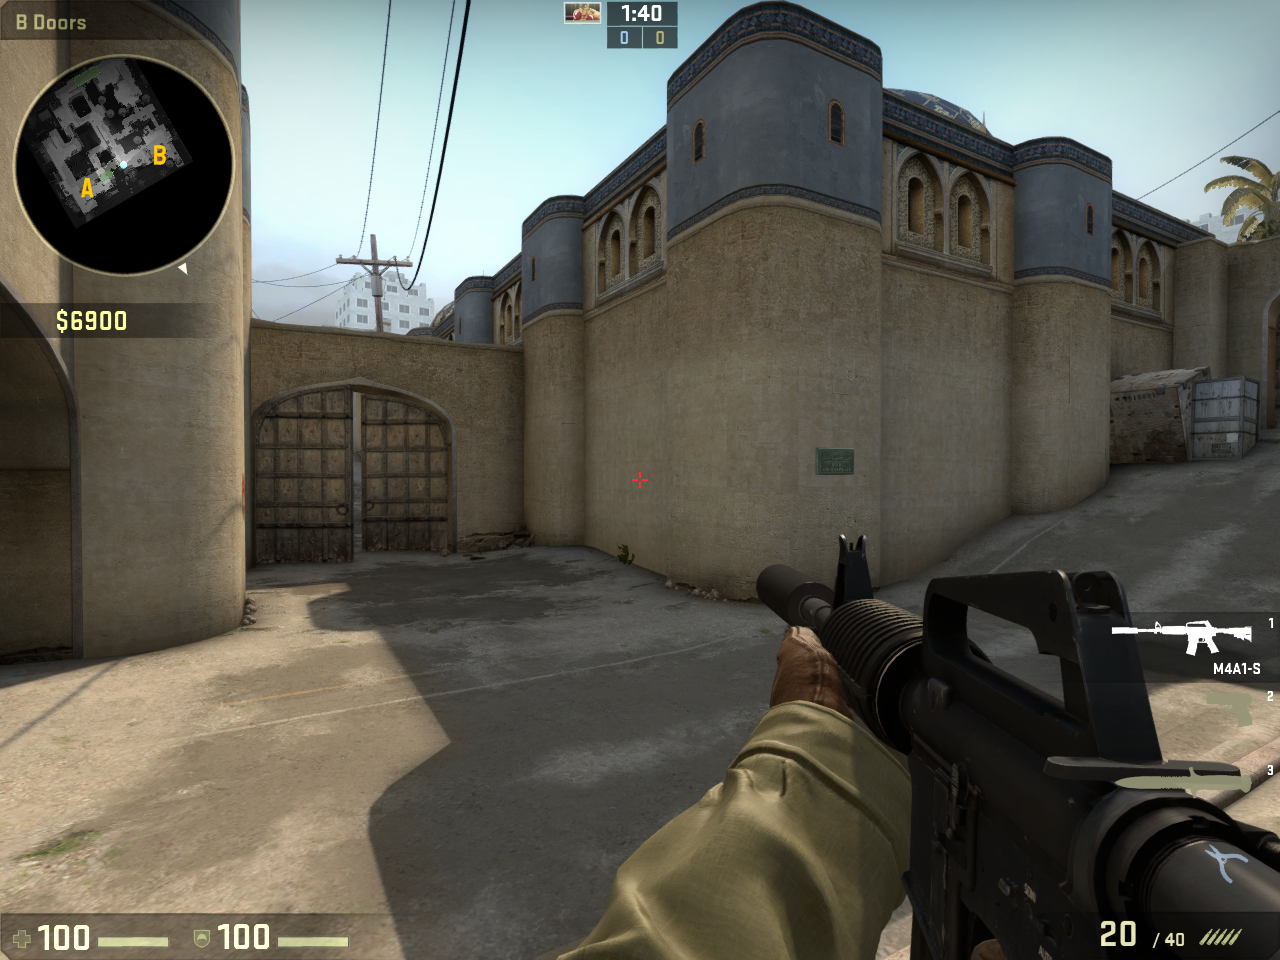
\includegraphics[width = 7cm]{billeder/CS_GO_4,3}
\caption{CS:GO med aspekt ratio 4:3}    
\label{CS_GO_4,3}}
\qquad
\begin{minipage}{9.33cm}
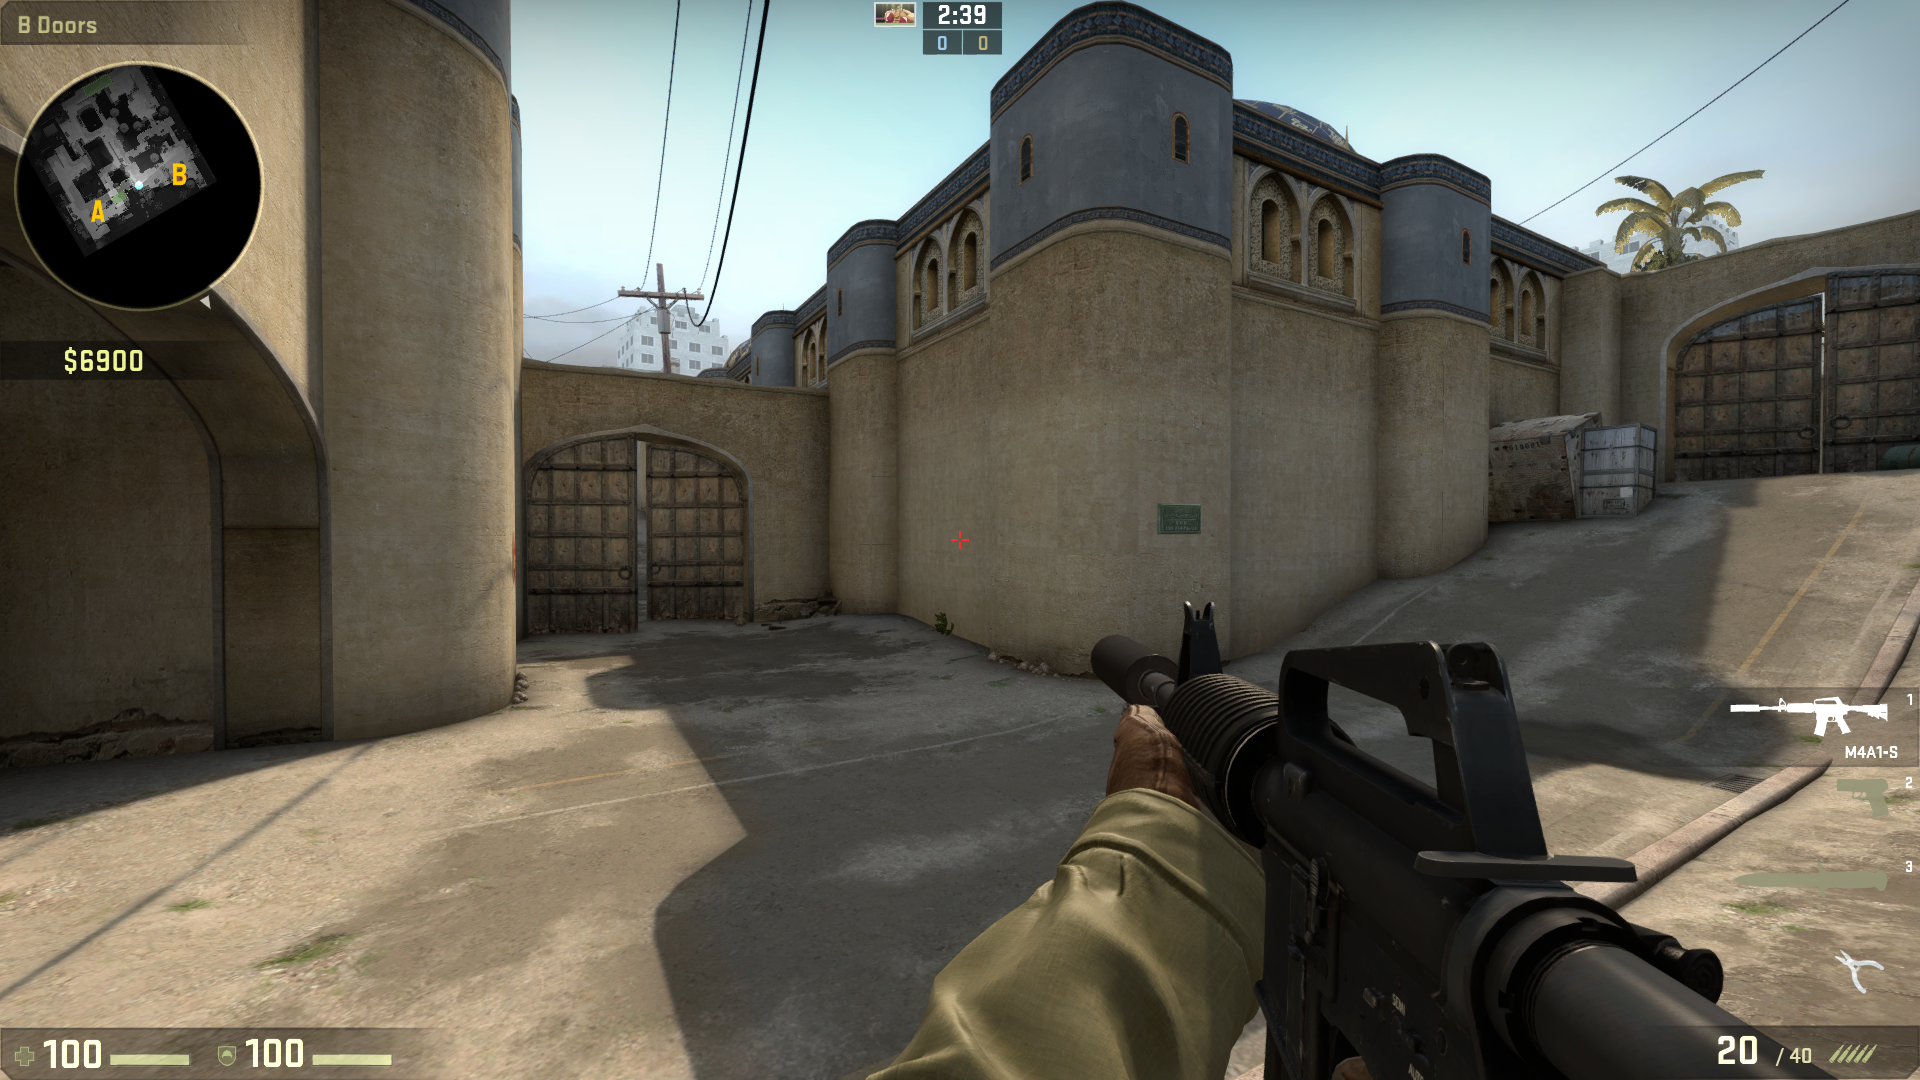
\includegraphics[width = 9.33cm]{billeder/CS_GO_16,9}
\caption{CS:GO med aspekt ratio 16:9}    
\label{CS_GO_16,9}
\end{minipage}
\end{figure} 

\section{Letterbox}

Den anden måde at komme uden om skaleringsproblemer på, er at tilføje sorte bars, også kaldet letterbox, til toppen og bunden af skærmen. På den måde tvinges spillet reelt set til at køre i et statisk aspekt ratio, og dermed er der ingen uretfærdigheder når det kommer til FOV \cite{computerhope}. Disse sorte bars kan også blive smidt på højre og venstre side af skærmen, og i disse tilfælde kaldes de pillarboxing \cite{Apple}. Nogle spil er nødt til at benytte sig af dette koncept, for at deres gameplay kan hænge sammen.

Et af disse spil er Speedrunners. Formålet med Speedrunners er at løbe om kap, og komme fremad hurtigst muligt, og dermed efterlade ens modstander bag sig. Alle fire spillere ser på den samme del af spilverdenen, og når at en spiller falder for langt bagefter, og kommer uden for skærmen, bliver spilleren elimineret. I det at spillet afhænger af at lose condition er at komme uden for skærmen, ville forskellige aspekt ratioer betyde at dem med et smallere FOV enten ville dø tidligere, eller vil være ude af stand til at se sin karakter mens han stadig er i live. Ved at tilføje letterboxes til spillere der ikke kører med et 16:9 aspekt ratio, sikre spillet sig at alle har det samme syn på spil verdenen, og der er enighed om hvornår at en spiller er ude af skærmen. På figur \ref{Speedrunners_16,9} ses spillet i det tiltænkte 16:9 aspekt ratio, og på figur \ref{Speedrunners_4,3} ses spillet i et 4:3 ratio hvor det er letterboxed.

\begin{figure}[h]
\centering
\parbox{7cm}{
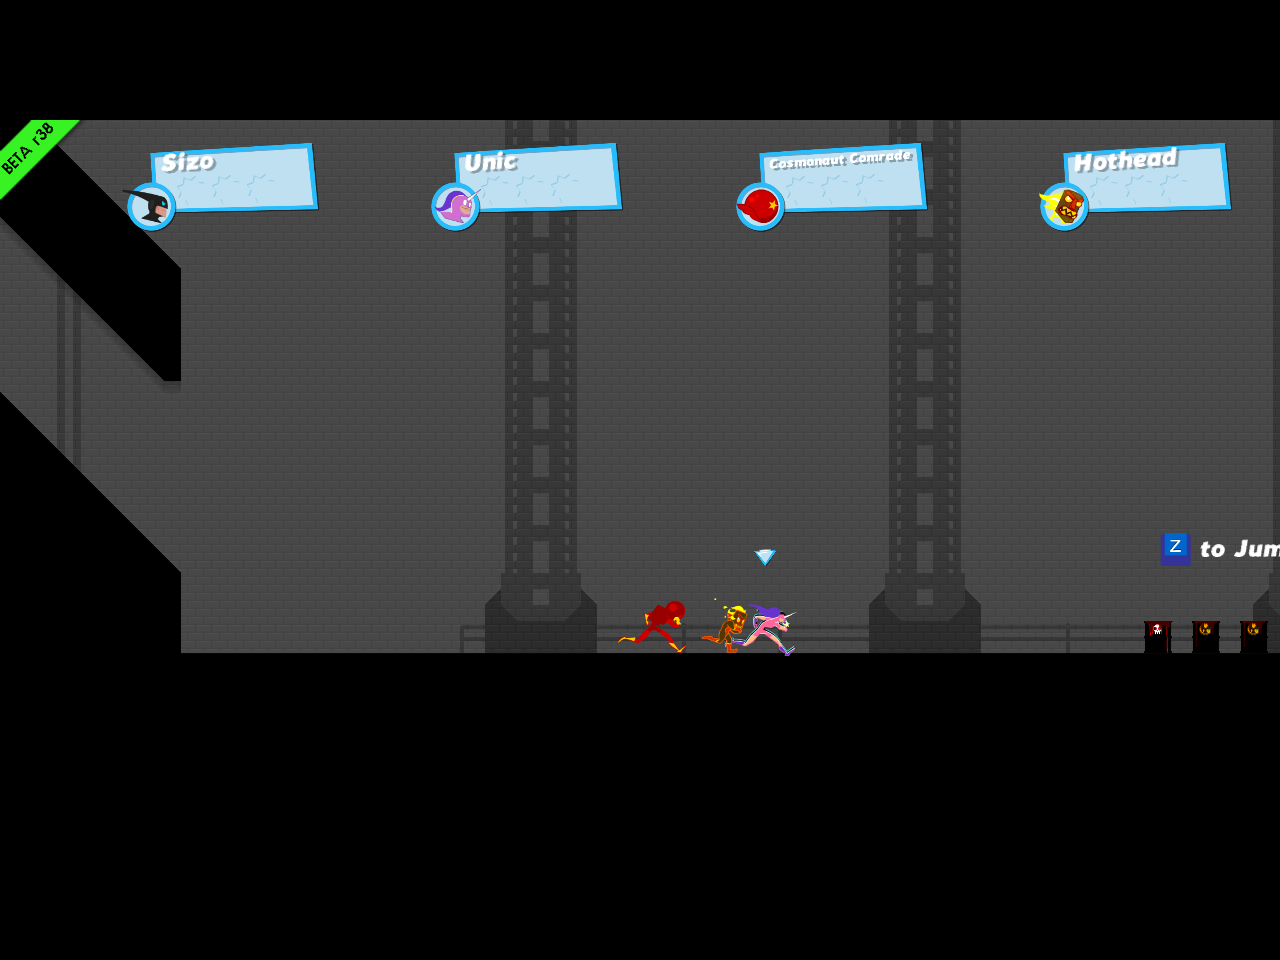
\includegraphics[width = 7cm]{billeder/Speedrunners_4,3}
\caption{Speedrunners med aspekt ratio 4:3}    
\label{Speedrunners_4,3}}
\qquad
\begin{minipage}{9.33cm}
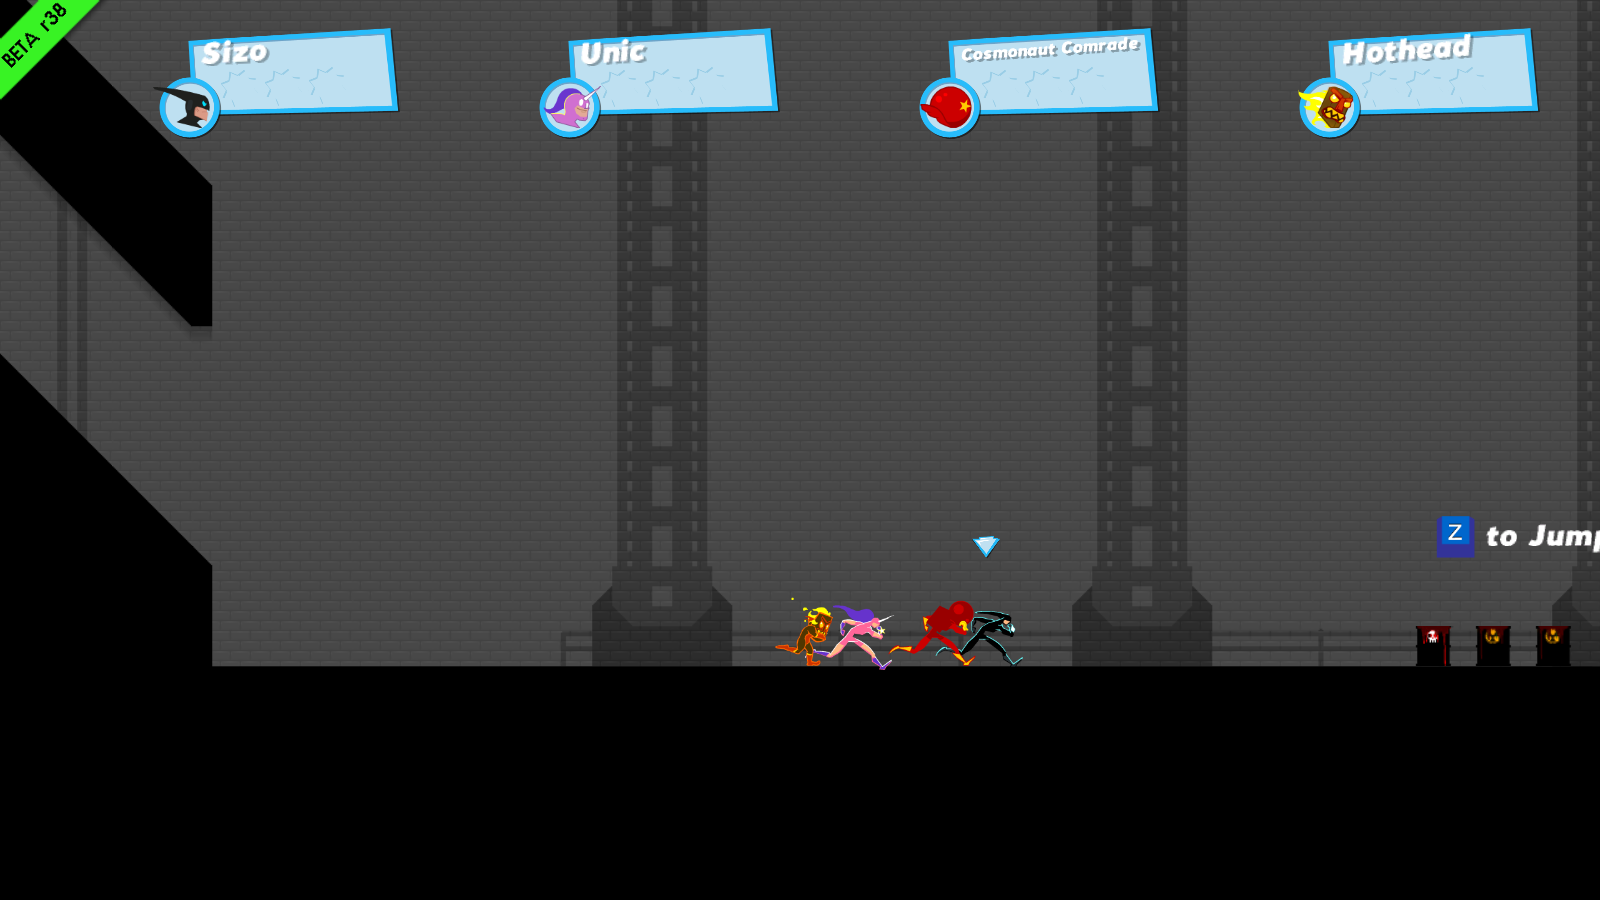
\includegraphics[width = 9.33cm]{billeder/Speedrunners_16,9}
\caption{Speedrunners med aspekt ratio 16:9}    
\label{Speedrunners_16,9}
\end{minipage}
\end{figure}

\section{Virtual viewport}

På mobilmarkedet findes der ligeledes mange forskellige aspekt ratios, og det bearbejdes i store træk på samme måde som på platforme med større displays. Det er dog i de færreste tilfælde at det er ønskeligt at tilføje letterboxes til mobil platformen, da der i forvejen ikke er meget plads at arbejde med, og det i desuden kan give et indtryk af at spillet ikke er beregnet til den brugte model.

En virtual viewport kan bruges til at vise en del af et environment, der kan justere sig selv efter dit aspekt ratio. Ved at lave en baggrund bred nok til at supportere et bredt aspekt ratio, og højt nok til at supportere et smalt et, kan man ved at tage udgangspunkt i midten af baggrunden, sikre at det vil give et godt indtryk på ethvert aspekt ratio. Dertil kan man sørge for at andre elementer på skærmen også justure sig selv efter kanterne af skærmen, for at sikre at de ikke bliver placeret på en måde der giver et upoleret indtryk \cite{gemserk}.

Dette koncept benyttes også på andre platforme. F.eks. har det online kortspil Hearthstone grafik der går ud over selve den kvadratiske brugerflade, således at grafikken på en widescreen skærm også giver et godt visuelt indtryk, uden et behov for at benytte sig af letterboxes i siderne. På figur \ref{Hearthstone_16,9} og \ref{Hearthstone_4,3} ses det hvordan Heartstone tilpasser sig den givne skærms aspekt ratio.
 
\begin{figure}[h]
\centering
\parbox{7cm}{
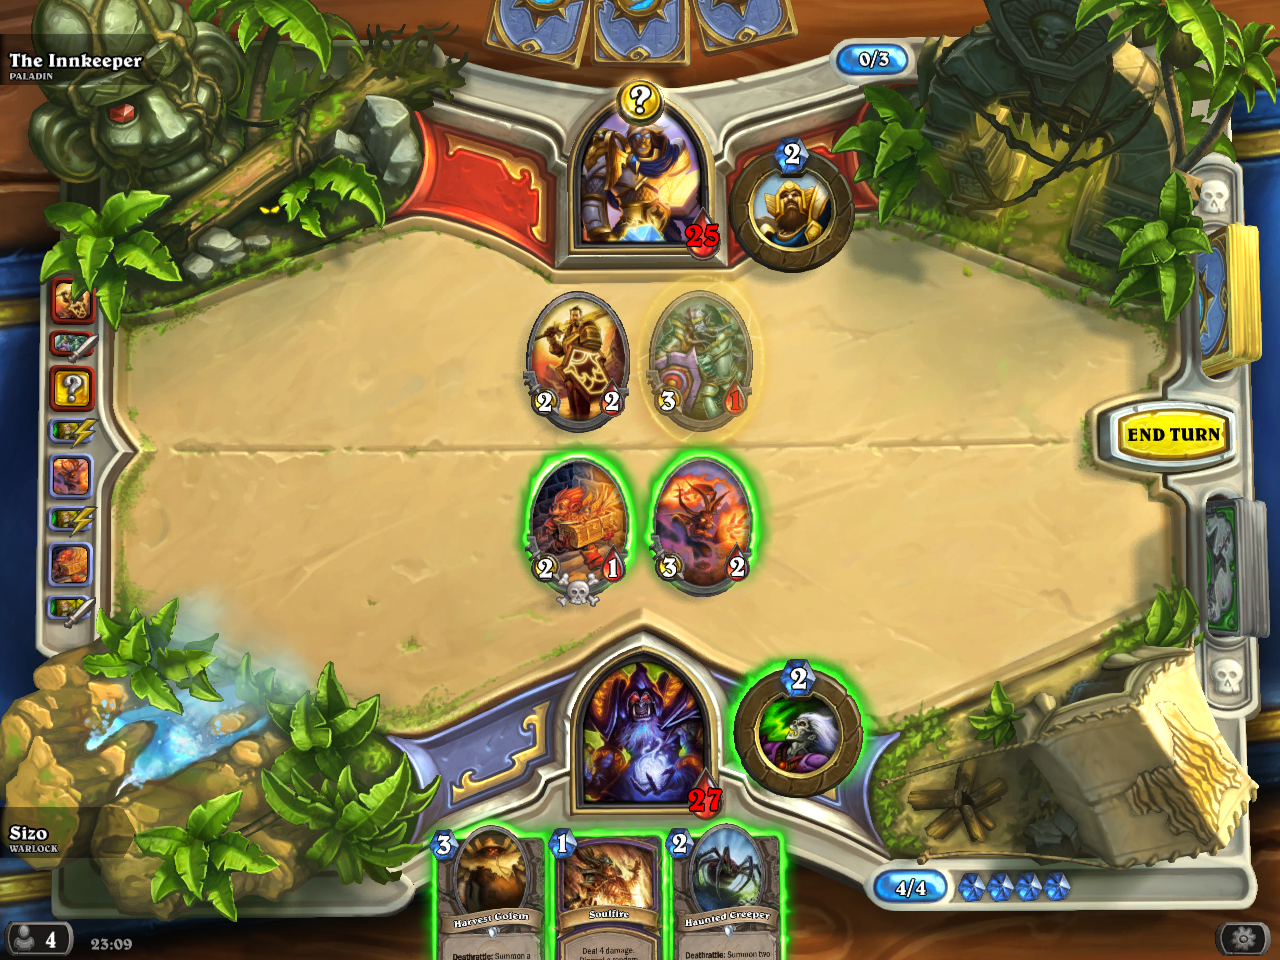
\includegraphics[width = 7cm]{billeder/Heathstone_4,3}
\caption{Hearthstone med aspekt ratio 4:3}
\label{Hearthstone_4,3}}
\qquad
\begin{minipage}{9.33cm}
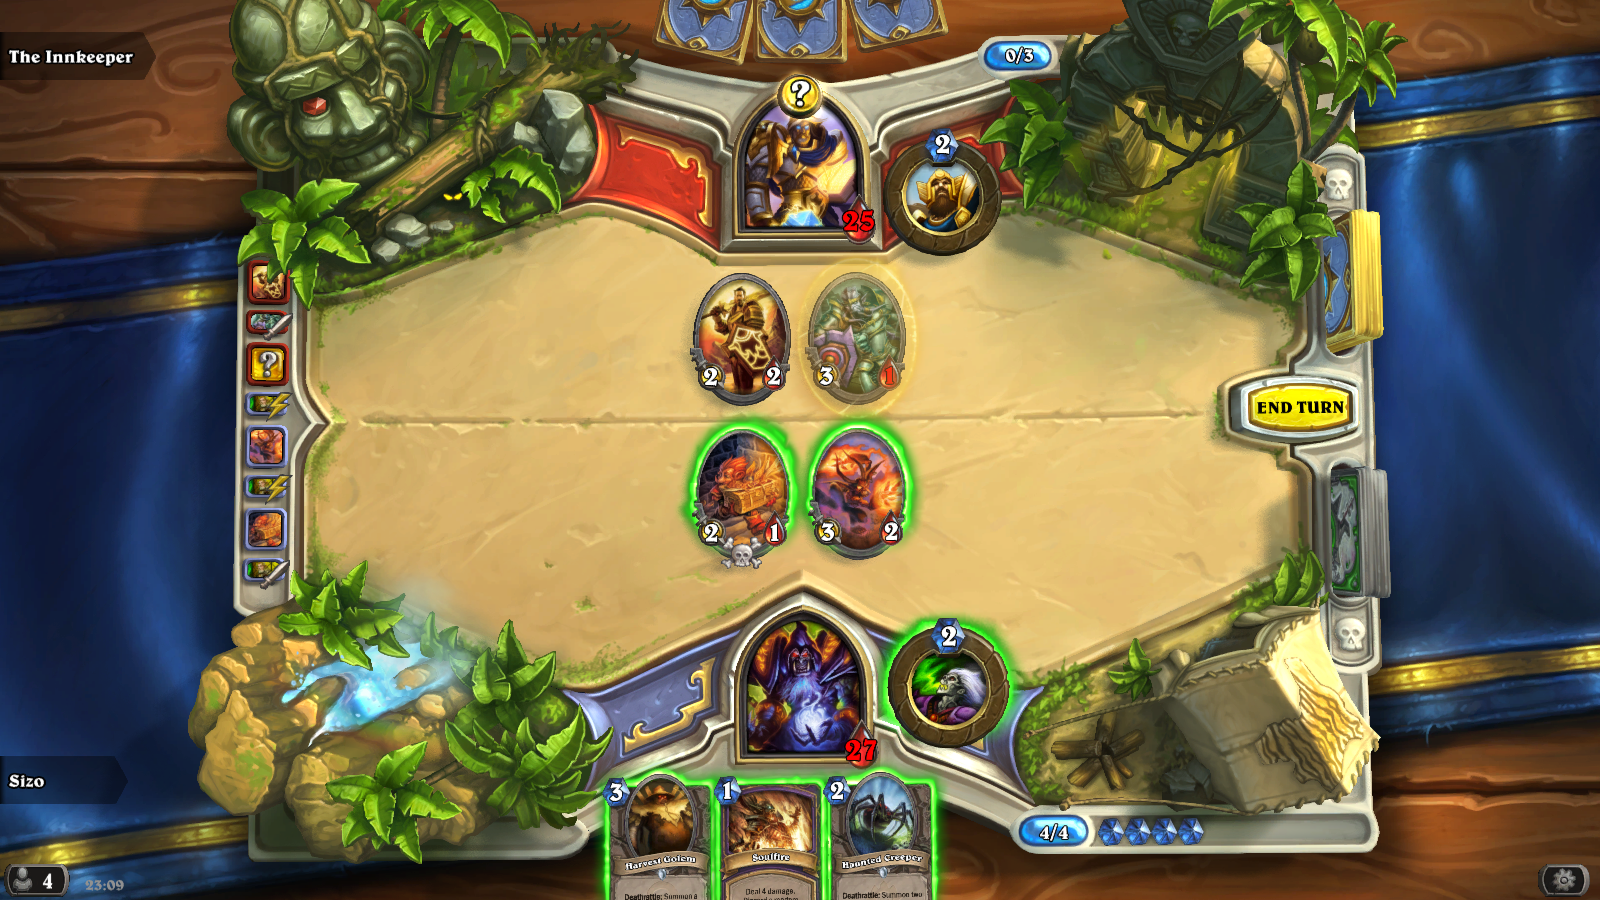
\includegraphics[width = 9.33cm]{billeder/Heathstone_16,9}
\caption{Hearthstone med aspekt ratio 16:9}
\label{Hearthstone_16,9}
\end{minipage}
\end{figure}
\end{document}